%%%%%
%  Page Geometry
%%%%%

\usepackage{geometry}
\geometry{margin=1in,headheight=1in}

%%%%%
%  Headers and Footers
%%%%%

\usepackage{fancyhdr}
\usepackage{transparent}
\pagestyle{fancy}
\fancyhf{}
\fancyhead[LO]{\transparent{0.4}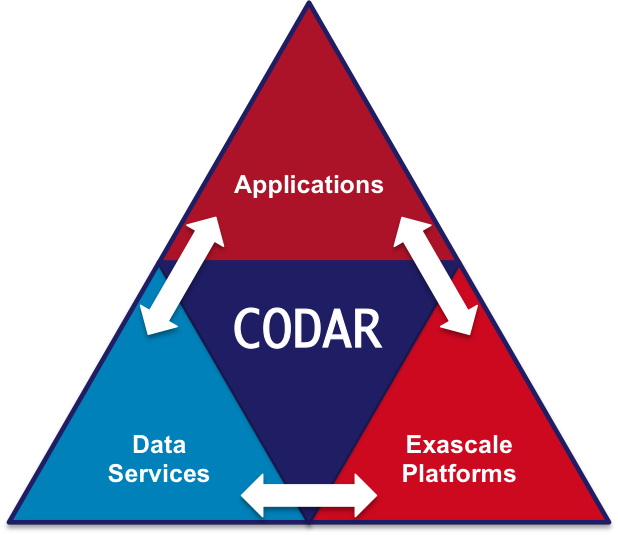
\includegraphics[height=0.4in]{Figs/CODAR.png}}
\fancyhead[RO]{\transparent{0.4}
\includegraphics[height=0.4in]{Figs/ecp.eps}}
\fancyfoot[CE,CO]{\thepage}
\fancyfoot[LE,LO]{\TITLE{}}
\fancyfoot[RE,RO]{Exascale Computing Project (ECP)}

%%%%%
%  Title Formating of Sections
%%%%%

\usepackage[explicit]{titlesec}

\titleformat{\section}
  {\normalfont\Large\bfseries}{\thesection}{1em}{#1}[{\titlerule[0.8pt]}]

\usepackage{titlesec}
\titlespacing{\section}{0pt}{*2}{*1.35}
\titlespacing{\subsection}{0pt}{*1.35}{*0.15}
%\titleformat{\subsection}[runin]{\bfseries}{\thesubsection}{1em}{}[.]

%\titleformat{ command }[ shape ]{ format }{ label }{ sep }{ before-code}
%\titleformat{\subsubsection}[runin]{\slshape}{\thesubsubsection}{1em}{}[.]
\titleformat{\subsubsection}[runin]{\bfseries}{\thesubsubsection}{1em}{#1}[.]
\titlespacing{\subsubsection}{0pt}{*0.105}{*1.00}

%\titleformat{\paragraph}[runin]{\bfseries}{\theparagraph}{1em}{}[.]
\titleformat{\paragraph}[runin]{\slshape}{\theparagraph}{1em}{#1}[.]
\titlespacing{\paragraph}{0pt}{*0.105}{*1.00}

\titleformat{\subparagraph}[runin]{}{\thesubparagraph}{1em}{\underline{#1}}[.]
%\titleformat{\subparagraph}[runin]{\bfseries}{\thesubparagraph}{1em}{}[.]
\titlespacing{\subparagraph}{0pt}{*0.105}{*1.00}

%%%%%
% Other packages
%%%%%

\usepackage{enumitem} % For tighter lists
\usepackage{cutwin,pstricks}
\usepackage{tcolorbox}

% Helvetica
% \renewcommand{\rmdefault}{phv}
% \renewcommand{\sfdefault}{phv}

\usepackage[font={footnotesize,bf}]{caption}

\usepackage{comment}
\usepackage{epsfig,wrapfig,url}
\usepackage[hidelinks]{hyperref}
\usepackage{pdfpages}
%\usepackage{amsfonts,amsmath,amscd,amsthm}
%\usepackage[mathscr]{euscript}
% Next line gives us superscript citations
%\usepackage[superscript,biblabel]{cite}
\usepackage{caption,subcaption}

\textfloatsep = 0.1in
\usepackage{array}
\newcolumntype{L}[1]{>{\raggedright\let\newline\\\arraybackslash\hspace{0pt}}m{#1}}
\usepackage{amsmath,amssymb}



\newif\iffinal

\finaltrue

\iffinal
  \newcommand\todo[1]{}
  \newcommand\ian[1]{}  
\else
  \newcommand\todo[1]{{\color{red}#1}}
  \newcommand\ian[1]{{\color{blue}[Ian: #1]}}
\fi

\setcounter{tocdepth}{2}
\setcounter{secnumdepth}{4}

\usepackage{listings} % for code listings

\newcommand\code[1]{{\tt #1}}

